\let\negmedspace\undefined
\let\negthickspace\undefined
\documentclass[journal]{IEEEtran}
\usepackage[a5paper, margin=10mm, onecolumn]{geometry}
\usepackage{lmodern} % Ensure lmodern is loaded for pdflatex
\usepackage{tfrupee} % Include tfrupee package

\setlength{\headheight}{1cm} % Set the height of the header box
\setlength{\headsep}{0mm}     % Set the distance between the header box and the top of the text

\usepackage{gvv-book}
\usepackage{gvv}
\usepackage{cite}
\usepackage{amsmath,amssymb,amsfonts,amsthm}
\usepackage{algorithmic}
\usepackage{graphicx}
\usepackage{textcomp}
\usepackage{xcolor}
\usepackage{txfonts}
\usepackage{listings}
\usepackage{enumitem}
\usepackage{mathtools}
\usepackage{gensymb}
\usepackage{comment}
\usepackage[breaklinks=true]{hyperref}
\usepackage{tkz-euclide} 
\usepackage{listings}
\usepackage{gvv}                                        
\def\inputGnumericTable{}                                 
\usepackage[latin1]{inputenc}                                
\usepackage{color}                                            
\usepackage{array}                                            
\usepackage{longtable}                                       
\usepackage{calc}                                             
\usepackage{multirow}                                         
\usepackage{hhline}                                           
\usepackage{ifthen}                                           
\usepackage{lscape}
\usepackage{xcolor}
\begin{document}

\bibliographystyle{IEEEtran}
\vspace{3cm}

\title{\textbf{\textcolor{red}{Hardware Assignment}}}

\author{PT-100 (AI-ML)}
\date{}

% \maketitle
% \newpage
% \bigskip

{\let\newpage\relax\maketitle}
\textbf{TRAINING DATA :}
\begin{table}[h]    	
    \centering
    \begin{tabular}{|c|c|} % Two centered columns
        \hline
        \textbf{Temperature ($^{\circ}$C)} & \textbf{Voltage (V)} \\ % Header row
        \hline
        25.2 & 4.604 \\ % Data rows
        \hline
        30.5 & 4.609 \\
        \hline
        54.1 & 4.637\\
        \hline
        62.7 & 4.647 \\
        \hline
        57.1 & 4.638 \\
        \hline
        81.6 & 4.653 \\
        \hline
        85.0 & 4.658 \\
        \hline
        90.2 & 4.663 \\
        \hline
        91.6 & 4.679\\
        \hline
        93.8 & 4.690 \\
        \hline
    \end{tabular}
 
    \caption{Training Data}
    \label{tab:1-1.9-6}
\end{table}
\\
\textbf{VALIDATION DATA :}
\begin{table}[h]
	\centering
	   \begin{tabular}{|c|c|} 
        \hline
        \textbf{Temperature ($^{\circ}$C)} & \textbf{Voltage (V)} \\
        \hline
        58.6 & 4.643 \\
        \hline
        65.3 & 4.649 \\
        \hline
        71.3 & 4.652 \\
        \hline
        78.7 & 4.661 \\
        \hline
        83.6 & 4.665 \\
        \hline
    \end{tabular}

	\caption{Validating Data}
	\label{tab:2-1.9-7}
\end{table}
\\
After training the \textbf{ARDIUNO}, the \textbf{Callendar-Van Dusen} equation comes out to be : \\
\begin{align}
	V(T) = 4.52171132 + \brak{2.01541525 \times 10^{-3}} T -\brak{8.15375669 \times 10^{-6}} T^2
\end{align}
\\
\begin{figure}[h]
	\centering
	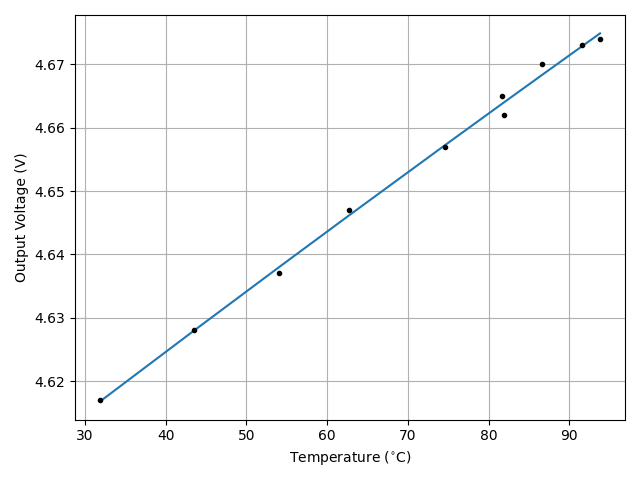
\includegraphics[width=0.75\textwidth]{figs/train.png}
    \caption{Training the Model}
    \label{fig:PT100}  
\end{figure}
\\
\newpage
\textbf{VALIDATION :}
\begin{figure}[ht]  
    \centering
    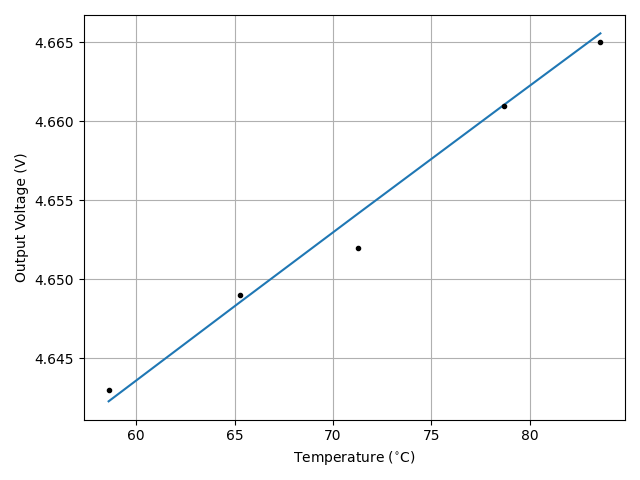
\includegraphics[width=0.8\textwidth]{figs/valid.png}  
    \caption{Validation}
    \label{fig:Valid}  
\end{figure}
\end{document}
